\documentclass[12pt,a4paper,oneside]{memoir}
\usepackage[utf8]{inputenc}
\usepackage[T1]{fontenc}
\usepackage{microtype}
\usepackage[dvips]{graphicx}
\usepackage{xcolor}
\usepackage{times}
\usepackage{ragged2e}

\usepackage[
breaklinks=true,colorlinks=true,
%linkcolor=blue,urlcolor=blue,citecolor=blue,% PDF VIEW
linkcolor=black,urlcolor=black,citecolor=black,% PRINT
bookmarks=true,bookmarksopenlevel=2]{hyperref}

\usepackage{biblatex}
\addbibresource{sample.bib}

\newenvironment{acknowledgement}%       New acknowledgement environment
    {\large\bfseries\centering ACKNOWLEDGEMENT%
    \par\medskip\normalfont\normalsize}%
    {}%

\newenvironment{candidate}%       New acknowledgement environment
    {\large\bfseries\centering CANDIDATE'S DECLARATION%
    \par\medskip\normalfont\normalsize}%
    {}%


\newenvironment{certificate}%       New acknowledgement environment
    {\large\bfseries\centering CERTIFICATE%
    \par\medskip\normalfont\normalsize}%
    {}%

\newenvironment{abs}%       New acknowledgement environment
    {\large\bfseries\centering ABSTRACT%
    \par\medskip\normalfont\normalsize}%
    {}%


\usepackage{titlesec}
\newcommand*{\justifyheading}{\raggedleft}
\titleformat{\chapter}[display]
  {\normalfont\Large\bfseries\justifyheading}{\chaptertitlename\ \thechapter}
  {10pt}{\vspace{1.5ex}}
  [\vspace{1ex}\titlerule]
\titlespacing*{\chapter}{-20pt}{-5pt}{10pt}



\usepackage{geometry}
% PDF VIEW
% \geometry{total={210mm,297mm},
% left=25mm,right=25mm,%
% bindingoffset=0mm, top=25mm,bottom=25mm}
% PRINT
\geometry{total={210mm,297mm},
left=20mm,right=20mm,
bindingoffset=10mm, top=25mm,bottom=25mm}

\OnehalfSpacing
%\linespread{1.3}

%%% CHAPTER'S STYLE
%\chapterstyle{bianchi}
%\chapterstyle{ger}
%\chapterstyle{madsen}
\chapterstyle{ntglike}
%\chapterstyle{ell}
%%% STYLE OF SECTIONS, SUBSECTIONS, AND SUBSUBSECTIONS
\setsecheadstyle{\bfseries\sffamily\raggedright}
\setsubsecheadstyle{\bfseries\sffamily\raggedright}
\setsubsubsecheadstyle{\bfseries\sffamily\raggedright}


%%% STYLE OF PAGES NUMBERING
%\pagestyle{companion}\nouppercaseheads 
%\pagestyle{headings}
%\pagestyle{Ruled}
\pagestyle{plain}
\makepagestyle{plain}
\makeevenfoot{plain}{\thepage}{}{}
\makeoddfoot{plain}{}{}{\thepage}
\makeevenhead{plain}{}{}{}
\makeoddhead{plain}{}{}{}

\setsecnumdepth{subsubsection}
\maxsecnumdepth{subsubsection} % chapters, sections, and subsections are numbered
\settocdepth{subsubsection}
\maxtocdepth{subsubsection} % chapters, sections, and subsections are in the Table of Contents


%%%---%%%---%%%---%%%---%%%---%%%---%%%---%%%---%%%---%%%---%%%---%%%---%%%

\begin{document}

%%%---%%%---%%%---%%%---%%%---%%%---%%%---%%%---%%%---%%%---%%%---%%%---%%%
%   TITLEPAGE
%
%   due to variety of titlepage schemes it is probably better to make titlepage manually
%
%%%---%%%---%%%---%%%---%%%---%%%---%%%---%%%---%%%---%%%---%%%---%%%---%%%
\thispagestyle{empty}

{%%%
\sffamily
\centering
\Large

~\vspace{\fill}

{\huge 
Voice dictation system for Punjabi language with cmu-sphinx speech recognition engine
}

\vspace{2.5cm}

{\LARGE
Satinderpal Singh
}

\vspace{3.5cm}

A thesis submitted in partial fulfillment for the\\
degree of Masters of Technology\\[1em]
in the\\[1em]
Sri Guru Granth Sahib World University, Fatehgarh Sahib

\vspace{3.5cm}

Supervisor: Prof. Vinay Bharadwaj

\vspace{\fill}

June 2015

%%%
}%%%

%\cleardoublepage
%%%---%%%---%%%---%%%---%%%---%%%---%%%---%%%---%%%---%%%---%%%---%%%---%%%
%%%---%%%---%%%---%%%---%%%---%%%---%%%---%%%---%%%---%%%---%%%---%%%---%%%
%-----------------------------------------------------------------------------------------------------------------------------------------------------
\newpage
\begin{candidate}
\addcontentsline{toc}{chapter}{Candidate's Declaration}
%\noindent\makebox[\linewidth]{\rule{\paperwidth}{1.0pt}}
\noindent\rule{17cm}{1.0 pt} \\

\justify
I hereby certify that I am student of M.Tech (regular) of Computer Science and engineering Department and declare that I own the full responsibility for the information, results etc. provided in this thesis titled \textbf{“Voice dictation system for Punjabi language with cmu-sphinx speech recognition engine”} Submitted to \textbf{Sri Guru Granth Sahib World University} for the award of \textbf{Master of Technology in Computer Science and Engineering} degree. I have taken care in all respect to honor the intellectual property right and have acknowledged the contributions of others for using them in this academic purpose. I further declare that in case of any violation of intellectual property right or copyright, I as a candidate will be fully responsible for the same. My supervisors and institute should not be held for full or partial violation of copy right if found at any stage of my degree.
\vspace{3 cm}

\noindent Place:  Fatehgarh Sahib   \hfill Satinderpal Singh \\
\noindent Date: \hfill Reg.No. 13012156
\end{candidate}
%---------------------------------------------------------------------------------------------------------------------------------------------------
\newpage
\begin{certificate}
\addcontentsline{toc}{chapter}{Certificate}
\noindent\rule{16cm}{1.0 pt} \\
\justify
This is to certify that the thesis work entitled \textbf{“Voice dictation system for Punjabi language with cmu-sphinx speech recognition engine”}, submitted by Satinderpal Singh, Reg. no 13012156 to the Sri Guru Granth Sahib World University, Fatehgarh Sahib, for the partial fulfillment of the requirement of the degree of Masters of Technology in Computer Science and Engineering is a record of student’s own study under my supervision and guidance. \\

This thesis has not been submitted to any other university or institution for the award of any other degree. \\
\vspace{3 cm}

\hfill \textbf{Supervisor}\\
\vspace{0 mm}
\hfill Mr. Vinay Bhardwaj \\
\vspace{0 mm}
\hfill Assistant Professor\\
\vspace{0 mm}
\hfill Department of Computer Science and Engg.\\
\vspace{0 mm}
\hfill SGGSWU, Fatehgarh Sahib\\
\vspace{2 cm}

The M.Tech Viva-Voice examination of \textbf{Satinderpal Singh} has been held on  \_\_\_\_\_\_. \\

\vspace{2 cm}

\noindent \textbf{Sign. of Supervisor}   \hfill \textbf{Sign. of External} \\
\noindent  \textbf{Examiner}  \\

\vspace{2 cm} 

\noindent  \textbf{Sign. of H.O.D} 

\end{certificate}

%---------------------------------------------------------------------------------------------------------------------------------------------------

\newpage
\begin{acknowledgement}
\addcontentsline{toc}{chapter}{Acknowledgement}
\noindent\rule{17cm}{1.0 pt} \\

\justify
First of all I would like to thank Almighty God. It’s only because of the blessings of the God that I have been able to complete my thesis work successfully. I would like to thank \textbf{Mr. Vinay Bhardwaj} for being my advisor, and for her guidance and support throughout my research work. I would also like to thank \textbf{Dr. H.S Rai} for helping me in choosing the research topic and guidance. I would also like to thank \textbf{Dr. Navdeep Kaur} Head of Department for her valuable suggestions about the research work. I am deeply grateful for all the help I have received during the course of this thesis at Sri Guru Granth Sahib World University, Fatehgarh sahib. I am also thankful to all the staff members of the CSE department and my friends specially \textbf{Jasleen Kaur} who have helped me in many ways directly or indirectly for this research work. \\

I would also like to show my gratitude to the \textbf{Peter Grasch} and \textbf{Nickolay Shmyrev} of cmu-sphinx community for sharing their pearls of wisdom with me during the course of this research. 


Finally I would like to thank my dear parents whose moral support and care always encouraged me to proceed.\\

\vspace{3 cm}

\hfill \textbf{Satinderpal Singh}

\end{acknowledgement}
%----------------------------------------------------------------------------------------------------------------------------------------------------
\newpage
\begin{abs}
\addcontentsline{toc}{chapter}{Abstract}
\noindent\rule{16cm}{1.0 pt} \\
\justify
This paper aims to discuss the implementation of Voice dictation(Voice-to-text) system for an Indian language Punjabi. The CMU-Sphinx toolkit based on Hidden Markov's Model(HMM), is used to develop the system. Initially, a language model is prerared with CMU-Sphinx toolkit and an acoustic model is prepared for the punjabi language. The system is trained with CMU-Sphinx trainer for distinct Punjabi words by collecting data from 3 speakers in real time environment. To make model platform independent a console based linux  environment is used for testing. The paper also describes the
role of each CMU-Sphinx tool, used in various phases of system development, by presenting a detailed architecture of dictation system developed using CMU-Sphinx library modules and tools. The experimental results show that the overall system performance is 94.09\%. 

\end{abs}
%\begin{abstract}
%\addcontentsline{toc}{chapter}{Abstract}
%   abstract-text
%\end{abstract}

\newpage


\tableofcontents*

\newpage
\listoffigures
\newpage
\listoftables
\clearpage




%%%---%%%---%%%---%%%---%%%---%%%---%%%---%%%---%%%---%%%---%%%---%%%---%%%
%%%---%%%---%%%---%%%---%%%---%%%---%%%---%%%---%%%---%%%---%%%---%%%---%%%

\chapter{INTRODUCTION}

\section{Content}
Natural Language Processing(NLP) is an area of research and application that explores how computers can be used to understand and manipulate natural language text or speech to do useful things. NLP researchers aim to gather knowledge on how human beings understand and use language so that appropriate tools and techniques can be developed to make computer systems understand and manipulate natural languages to perform the desired tasks. The foundations of NLP lie in a number of disciplines, viz. computer and information sciences, linguistics, mathematics, electrical and electronic engineering, artificial intelligence and robotics, psychology, etc. Applications of NLP include a number of fields of studies, such as machine translation, natural language text processing and summarization, user interfaces, multilingual and cross language information retrieval(CLIR), speech recognition, artificial intelligence and expert systems, and so on [1].

At the core of any NLP task there is the important issue of natural language understanding. The process of building computer programs that understand natural language involves three major problems: the first one relates to the thought process, the second one to the representation and meaning of the linguistic input, and the third one to the world knowledge. Thus, an NLP system may begin at the word level – to determine the morphological structure, nature(such as part-of- speech, meaning) etc. of the word – and then may move on to the sentence level – to determine morphological level that deals with the smallest parts of words, that carry a meaning, and suffixes and prefixes:-  lexical level that deals with lexical meaning of words and parts of speech analyses, syntactic level that deals with grammar and structure of sentences, semantic level that deals with the meaning of words and sentences, discourse level that deals with the structure of different kinds of text using document structures and pragmatic level that deals with the knowledge that comes from the outside world, i.e. from outside the contents of the document.

The goal of automatic speech recognition is to develop technique and system that enables computers to accept speech input. NLP is a field of computer science and linguistics concerned with the interactions between computers and human(natural) languages. In theory, natural-language processing is a very attractive method of human-computer interaction. Natural-language understanding is sometimes referred to as an AI-complete problem, because natural-language recognition seems to require extensive knowledge about the outside world and the ability to manipulate it.

NLP is an area of research and application that explores how computers can be used to understand and manipulate natural language text or speech to do useful things. NLP researchers aim to gather knowledge on how human beings understand and use language so that appropriate tools and techniques can be developed to make computer systems understand and manipulate natural languages to perform the desired tasks. The foundations of NLP lie in a number of disciplines, disciplines, viz. computer and information sciences, linguistics, mathematics, electrical and electronic engineering, artificial intelligence and robotics, psychology, etc.Research in natural language processing has been going on for several decades dating back to the late 1940s. Machine translation(MT) was the first computer-based application related to natural language.

Natural language processing approaches fall roughly into four categories: symbolic, statistical, connectionist, and hybrid. Symbolic and statistical approaches have coexisted since the early days of this field. Connectionist NLP work first appeared in the 1960’s. For a long time, symbolic approaches dominated the field. In the 1980’s, statistical approaches regained popularity as a result of the availability of critical computational resources and the need to deal with broad, real- world contexts. Connectionist approaches also recovered from earlier criticism by demonstrating the utility of neural networks in NLP.

Speech is a complex phenomenon. It is important to  understand how is it produced and perceived. The naive perception is often that speech is built with words, and each word consists of phones. The reality is unfortunately very different. Speech is a dynamic process without clearly distinguished parts.

\subsection{Structure of Speech}
Speech is a continuous audio stream where rather stable states mix with dynamically changed states. In this sequence of states, one can define more or less similar classes of sounds, or phones. Words are understood to be built of phones, but this is certainly not true. The acoustic properties of a waveform corresponding to a phone can vary greatly depending on many factors - phone context, speaker, style of speech and so on. The so called coarticulation makes phones sound very different from their “canonical” representation. Next, since transitions between words are more informative than stable regions, developers often talk about diphones- parts of phones between two consecutive phones. Sometimes developers talk about subphonetic units - different substates of a phone. Often three or more regions of a different nature can easily be found [2].

The first part of the phone depends on its preceding phone, the middle part is stable, and the next part depends on the subsequent phone. That's why there are often three states in a phone selected for speech recognition.Sometimes phones are considered in context. Such phones in context are called triphones or even quinphones. For computational purpose it is helpful to detect parts of triphones instead of triphones as a whole, for example, to create a detector for a beginning of triphone and share it across many triphones. The whole variety of sound detectors can be represented by a small amount of distinct short sound detectors. Usually we use 4000 distinct short sound detectors to compose detectors for triphones. We call those detectors senones. 

\section{ Problem Statement}

In this thesis work, the problem formulation for Punjabi Dictation in Natuarl Language Processing is defined. It would lead to the development of the system for the Punjab language model and Gurmuki font so that the speech to text covergence softwares and systems could convert speech data into Gurmukhi font. As the speech to text convergence is available for the some internationl language, but are not available for punjabi language and Gurmukhi font. The model used for this purpose is HMM(Hidden Markov’s MOdel) along with the CMUSphinx toolkit which are responsible for speech recognization and storing the data to the database. Further many liberaries are available for defining the new Acoustic Model for the different languages, so, we would use one of these model for defining language model for our requirement. The output of the data may be extracted through terminal using ANSI terminal protocol [3].

\section{Aims and Objectives}

\begin{itemize}
  \item[$\bullet$] Our main objective is to develop an application for Punjabi Dictation.
  \item[$\bullet$] Make decision about the use of specific library and software.
  \item[$\bullet$] Construct database for the words in Punjabi. 
  \item[$\bullet$] Construct database for the speech in Punjabi. 
  \item[$\bullet$] Develop a Language Model for Punjabi language.	
\end{itemize}

\section{Organization of the Thesis}
The reminder of thesis is organized as:

In \textbf{Chapter 2}, we need to have introduction of fundamentals of Speech recognition and Dictation and its challenges. Also characteristics, advantages of Speech-to-Text are discussed. Dictation performance and issues are described. Then CMUSphinx, Hidden Markov's Model are described.\\

In \textbf{Chapter 3}, we cover the literature review of our topic.\\


In \textbf{Chapter 4}, we cover the proposed scheme of our topic which includes motivation and basic design of our that are related to our topic.\\


In \textbf{Chapter 5}, we deal with experimental results and analysis of our work. This section describes the tools and platform used in our project.
The tool used in our project is CMULTK and plate form used is Linux and operating system is UBUNTU 14.04.\\


In \textbf{Chapter 6}, covers the conclusion by us. At last we have shown different references including research papers, websites and books which we have gone through during my projects. 







%===================================================================================================================================================






\chapter{ CONCEPTS OF SPEECH}

\section{Introduction}
Speech is a complex phenomenon. People rarely understand how is it produced and perceived. The naive perception is often that speech is built with words, and each word consists of phones. The reality is unfortunately very different. Speech is a dynamic process without clearly distinguished parts. It's always useful to get a sound editor and look into the recording of the speech and listen to it. Here is for example the speech recording in an audio editor.

\begin{figure}[h]
    \centering
    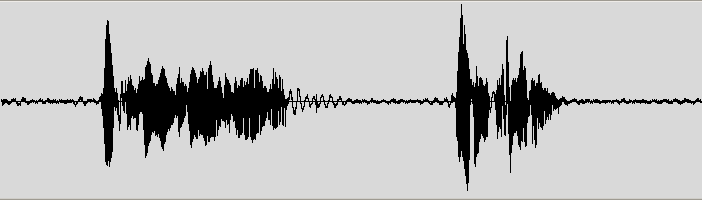
\includegraphics[scale=0.5]{waveform}
    \caption{Speech Waveform}
%    \label{fig:mesh1}
\end{figure}

All modern descriptions of speech are to some degree probabilistic. That means that there are no certain boundaries between units, or between words. Speech to text translation and other applications of speech are never 100 percent correct. That idea is rather unusual for software developers, who usually work with deterministic systems. And it creates a lot of issues specific only to speech technology [4]. 


\subsection{Concept of Speech}
Speech is a continuous audio stream where rather stable states mix with dynamically changed states. In this sequence of states, one can define more or less similar classes of sounds, or phones. Words are understood to be built of phones, but this is certainly not true. The acoustic properties of a waveform corresponding to a phone can vary greatly depending on many factors - phone context, speaker, style of speech and so on. The so called coarticulation makes phones sound very different from their “canonical” representation. Next, since transitions between words are more informative than stable regions, developers often talk about diphones- parts of phones between two consecutive phones. Sometimes developers talk about subphonetic units - different substates of a phone. Often three or more regions of a different nature can easily be found [5].

The first part of the phone depends on its preceding phone, the middle part is stable, and the next part depends on the subsequent phone. That's why there are often three states in a phone selected for speech recognition.Sometimes phones are considered in context. Such phones in context are called triphones or even quinphones. For computational purpose it is helpful to detect parts of triphones instead of triphones as a whole, for example, to create a detector for a beginning of triphone and share it across many triphones. The whole variety of sound detectors can be represented by a small amount of distinct short sound detectors. Usually we use 4000 distinct short sound detectors to compose detectors for triphones. We call those detectors senones. 


\subsection{Recognition Precess}
 The common way to recognize speech is the following: we take waveform, split it on utterances by silences then try to recognize what's being said in each utterance. To do that we want to take all possible combinations of words and try to match them with the audio. We choose the best matching combination. There are few important things in this match [6].

First of all it's a concept of features. Since number of parameters is large, we are trying to optimize it. Numbers that are calculated from speech usually by dividing speech on frames. Then for each frame of length typically 10 milliseconds we extract 39 numbers that represent the speech. That's called eature vector. They way to generates numbers is a subject of active investigation, but in simple case it's a derivative from spectrum.

Second it's a concept of the model. Model describes some mathematical object that gathers common attributes of the spoken word. In practice, for audio model of senone is gaussian mixture of it's three states - to put it simple, it's a most probable feature vector. From concept of the model the following issues raised - how good does model fits practice, can model be made better of it's internal model problems, how adaptive model is to the changed conditions.

The model of speech is called Hidden Markov Model or HMM, it's a generic model that describes black-box communication channel. In this model process is described as a sequence of states which change each other with certain probability. This model is intended to describe any sequential process like speech. It has been proven to be really practical for speech decoding.

Third, it's a matching process itself. Since it would take a huge time more than universe existed to compare all feature vectors with all models, the search is often optimized by many tricks. At any points we maintain best matching variants and extend them as time goes producing best matching variants for the next frame.

\subsubsection{Models}
According to the speech structure, three models are used in speech recognition to do the match:
\begin{description}
%  \item[$\cdot$ bla1] item 1
  \item[$\bullet$ Acoustic Model] contains acoustic properties for each senone. There are context-independent models that contain properties (most probable feature vectors for each phone) and context-dependent ones (built from senones with context). 
%  \item[$\ast$ bla3] item 3
  \item[$\bullet$ Phonetic Dictionary]
contains a mapping from words to phones. This mapping is not very effective. For example, only two to three pronunciation variants are noted in it, but it's practical enough most of the time. The dictionary is not the only variant of mapper from words to phones. It could be done with some complex function learned with a machine learning algorithm. 

  \item[$\bullet$ Language Model]
	is used to restrict word search. It defines which word could follow previously recognized words (remember that matching is a sequential process) and helps to significantly restrict the matching process by stripping words that are not probable. Most common language models used are n-gram language models-these contain statistics of word sequences-and finite state language models-these define speech sequences by finite state automation, sometimes with weights. To reach a good accuracy rate, your language model must be very successful in search space restriction. This means it should be very good at predicting the next word. A language model usually restricts the vocabulary considered to the words it contains. That's an issue for name recognition. To deal with this, a language model can contain smaller chunks like subwords or even phones. Please note that search space restriction in this case is usually worse and corresponding recognition accuracies are lower than with a word-based language model [7].

\end{description}

\begin{figure}[h]
    \centering
    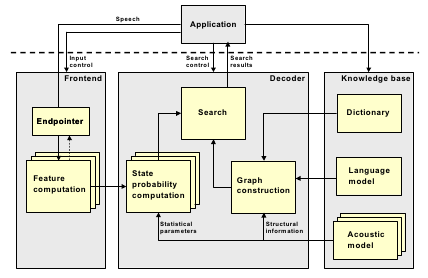
\includegraphics[scale=1.0]{sphinx4_architecture}
    \caption{Sphinx Architecture}
%    \label{fig:mesh1}
\end{figure}


Most current speech recognition systems use hidden Markov models(HMMs) to deal with the temporal variability of speech and Gaussian mixture models(GMMs) to deter- mine how well each state of each HMM fits a frame or a short window of frames of coefficients that repre- sents the acoustic input. An alternative way to evaluate the fit is to use a feed-forward neural network that takes several frames of coefficients as input and produces posterior probabilities over HMM states as output.

PocketSphinx is a flexible, modular and pluggable framework to help foster new innovations in the core research of hidden Markov model(HMM) speech recognition systems. The design of PocketSphinx is based on patterns that have emerged from the design of past systems as well as new requirements based on areas that researchers currently want to explore. To exercise this framework, and to provide researchers with a “research- ready” system, Sphinx-4 also includes several implementations of both simple and state-of-the-art techniques. The framework and the implementations are all freely available via open source.

PocketSphinx is a flexible, modular and pluggable framework to help foster new innovations in the core research of hidden Markov model (HMM) speech recognition systems. The design of PocketSphinx is based on patterns that have emerged from the design of past systems as well as new requirements based on areas that researchers currently want to explore. To exercise this framework, and to provide researchers with a “research- ready” system, Sphinx-4 also includes several implementations of both simple and state-of-the-art techniques. The framework and the implementations are all freely available via open source.

When researchers approach the problem of core speech recognition research, they are often faced with the problem of needing to develop an entire system from scratch, even if they only want to explore one facet of the field. Open source speech recognition systems are available, such as HTK , ISIP , AVCSR  and earlier versions of the Sphinx systems. The available systems are typically optimized for a single approach to speech system design. As a result, these systems intrinsically create barriers to future research that departs from the original purpose of the system.  First and foremost, PocketSphinx is a modular and pluggable framework that incorporates design patterns from existing systems, with sufficient flexibility to support emerging areas of research interest. The framework is modular in that it comprises separable components dedicated to specific tasks, and it is pluggable in that modules can be easily replaced at run time. To exercise the framework, and to provide researchers with a working system, PocketSphinx also includes a variety of modules that implement state-of-the-art speech recognition techniques.


\section{Advantages of Speech Recognition and Dictation systems}

\begin{itemize}
  \item[$\bullet$] Speech is a very natural way to interact, and it is not necessary to sit at a keyboard or work with a remote control.
  \item[$\bullet$] No training required for users.
  \item[$\bullet$] With speech recognition software, become a lot more productive – you’ll be able to get your work done much more quickly.
  \item[$\bullet$] Most of us can dictate at least 3 times faster than we can type. 
  \item[$\bullet$] It’s like having your own Personal Assistant available 24/7.	
\end{itemize}

\section{Principles of HMM}
Speech recognition systems generally assume that the speech signal is a realisation of some mes-sage encoded as a sequence of one or more symbols. To effect the reverse operation of recognising the underlying symbol sequence given a spoken utterance, the continuous speech waveform is first converted to a sequence of equally spaced discrete parameter vectors. This sequence of parameter vectors is assumed to form an exact representation of the speech waveform on the basis that for the duration covered by a single vector (typically 10ms or so), the speech waveform can be regarded as being stationary. Although this is not strictly true, it is a reasonable approximation. Typical parametric representations in common use are smoothed spectra or linear prediction coefficients plus various other representations derived from these. 

The role of the recogniser is to effect a mapping between sequences of speech vectors and the wanted underlying symbol sequences. Two problems make this very difficult. Firstly, the mapping from symbols to speech is not one-to-one since different underlying symbols can give rise to similar speech sounds. Furthermore, there are large variations in the realised speech waveform due to speaker variability, mood, environment, etc.  Secondly, the boundaries between symbols cannot be identified explicitly from the speech waveform. Hence, it is not possible to treat the speech waveform as a sequence of concatenated static patterns. 

The second problem of not knowing the word boundary locations can be avoided by restricting the task to isolated word recognition. This implies that the speech waveform corresponds to a single underlying symbol (e.g. word) chosen from a fixed vocabulary. Despite the fact that this simpler problem is somewhat artificial, it nevertheless has a wide range of practical applications. Furthermore, it serves as a good basis for introducing the basic ideas of HMM-based recognition before dealing with the more complex continuous speech case. Hence, isolated word recognition using HMMs will be dealt with first.

\begin{figure}[h]
    \centering
    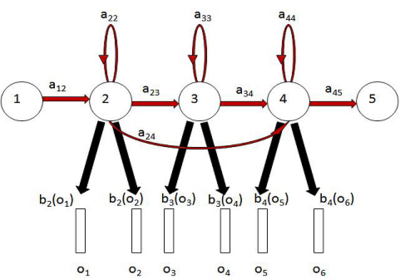
\includegraphics[scale=1.0]{400px-Mfcc_fig5}
    \caption{The Markov Generation Model}
%    \label{fig:mesh1}
\end{figure}


\section{Application of Speech Recognition}

\begin{description}
  \item[$\bullet$ Automation of Operator Services] Systems like the Voice Recognition Call Processing (VRCP) system introduced by AT and T or the Automated Alternate Billing System (AABS) introduced by Nortel enabled operator functions to be handled by speech recognition systems. The VRCP system handled so-called ‘operator assisted’ calls such as Collect, Third Party Billing, Person-to- Person, Operator Assisted Calling, and Calling Card calls. The AABS system automated the acceptance (or rejection) of billing charges for reverse calls by recognizing simple variants of the two word vocabulary Yes and No.
  \item[$\bullet$ Automation of Directory Assistance]  Systems were created for assisting operators with the task of determining telephone numbers in response to customer queries by voice. Both NYNEX and Nortel introduced a system that did front end city name recognition so as to reduce the operator search space for the desired listing, and several experimental systems were created to complete the directory assistance task by attempting to recognize individual names in a directory of as many as 1 million names. Such systems are not yet practical (because of the confusability among names) but for small directories, such systems have been widely used (e.g. in corporate environments).
  \item[$\bullet$ Voice Dialing] Systems have been created for voice dialing by name (so- called alias dialing such as Call Home, Call Office) from AT and T, NYNEX, and Bell Atlantic, and by number (ATandT SDN/NRA) to enable customers to complete calls without having to push buttons associated with the telephone number being called.
  \item[$\bullet$ Voice Banking Services] A system for providing access to customer accounts, account balances, customer transactions, etc. was first created in Japan by NTT (the ANSER System) more than 10 years ago in order to provide a service that was previously unavailable. Equivalent services have been introduced in banks worldwide over the last several years. 
  \item[$\bullet$ Voice Prompter]A system for providing voice replacement of touch-tone input for so-called Interactive Voice Response (IVR) systems was introduced by AT and T in the early 1990’s (initially in Spain because of the lack of touch- tone phones in that country). This system initially enabled the customer to speak the touch-tone position (i.e. speak or press the digit one); over time systems have evolved so that customers can speak the service associated with the touch-tone position (e.g. say reservations or push the 1-key, say schedule or push the 2-key, etc. 
  \item[$\bullet$ Directory Assistance Call Completion] This system was introduced by both AT and T and NYNEX to handle completion of calls made via requests for Directory Assistance. Since Directory Assistance numbers are provided by an independent system, using Text-to-Speech synthesis to speak out the listing, speech recognition can be used to reliably recognize the listing and dial the associated number. This highly unusual use of a speech recognizer to interface with a speech synthesizer is one of the unusual outgrowths of the fractionation of the telephone network into local and long distance carriers in the United State.
  \item[$\bullet$ Reverse Directory Assistance] This system was created by NYNEX:, Bellcore, and Ameritech to provide name and address information associated with a spoken telephone number.Information Services. These type of systems enable customers to access information lines to retrieve information about scores of sportilng events, traffic reports, weather reports, theatre bookings, restaurant reservations, etc. 
  \item[$\bullet$ Agent Technology] Systems like Wildfire and Maxwell (AT and T) enable customers to interact with intelligent agents via voice dialogues in order to manage calls (both in-coming and out-going calls), manage mesaages (both voice and email), get information from the Web (eg, movie reviews, calling directories), customize services (e.g., first thing each morning the agent provides the traffic and weather reports), personalize services (via the agent personality, speed, helpfulness), and adapt to user preferences (e.g., learn how the user likes to do things and react appropriate.
  \item[$\bullet$ Customer Care] The goal of customer care systems is to replace Interactive Voice Response systems with a dialogue type of interaction to make it easier for the user to get the desired help without having to navigate complicated menus or understand the terminology of the place being called for ihelp. The How May I Help You (HMIHY) customer care system of AT and T is an excellent example of this type of system.
  \item[$\bullet$ Computer Telephony Integration] Since the telecommunication network of the future will integrate the telephony (POTS) and computer (Packet) networks, a range of new applications will arise which exploit this integration more fully. One prime example is registry services where the network locates the user and determines the most appropriate way to communicate with them. Another example is providing a user cache of the most frequently accessed people in order to provide a rapid access mechanism for these frequently called numbers.
  \item[$\bullet$ Voice Dictation]  Although the desktop already supports voice dictation of documents, a prime telecommunications application of speech recognition would be for generating voice responses to email queries so that the resulting message becomes an email message back to the sender (rather than a voice mail response to an email message).
\end{description}

\section{Summary}
In this chapter, we describes about the Introduction of Speech Recognition concept. Then further we discussed about Hidden mrkov's Model. In chapter we discussed about advantages of Speech Recognition systems, application of Speeh Recognition System.

%==============================================================================================================================================
\chapter{LITERATURE REVIEW}
\section{Literature Review}
The main objective of the present study was: “To develop a software for speech to
text conversion”. The researcher had studied a lot of related literature to identify the
different works done in the related area. The study had given a more clear vision in
the task. In this present chapter, the brief information about the related research works
for the present study is given.
\subsection{A glance over Related Literature}
Initial computers were design just to do simple calculations; scientists have been
trying to endow the computer with more and more intelligence. That is to make the
digital machine, do things, which require human-like intelligence. Thus the term
Artificial Intelligence (AI) was coined in early 1950s. Gradually scientists came to
know the immense power of the device and its limitations. More and more systems
have been developed as a consequence of incremental advances in computer science.
Slowly these electronics devices have been spreading their roots in the soils of this
society. Now computer systems are available for applications of civil amenities to
medical diagnosis; home entertainment to space programs; simple calculations to
complex mathematical modeling etc [7].

In today’s fast placed world where every human being has to combat a race against
time – a direct interface between the spoken words and computer user will gleefully
accept the same words spontaneously typed on the computer screen with minimum
lapse of time. The phenomenon is known as speech (voice) recognition.

Speech recognition is an emerging technology where a speaker speaks to computer
with the microphone and computer understands the given words. Speech recognition
is a great supplement to traditional mouse and keyboard input; it will boost
productivity and provide a new option for people who have difficulty using a
keyboard.

Speech is the most common mode of communication among human beings. The
objective of speech recognition is to recognize the message being spoken. Differentorganization and researchers define the term “speech recognition”, and it can be summarized as follow:
\begin{description}
\item[$\bullet$] Speech recognition extracts the message information in a speech signal to control the
actions of a machine in response to spoken commands.
\item[$\bullet$]Speaker recognition identifies or verifies a speaker for restricting access to
information, network or physical premises [7].
\item[$\bullet$]Speech recognition is the process of finding a linguistic interpretation of a spoken
utterance, typically, this means finding the sequence of characters, which forms the
word.
\end{description}

\subsection{Some Empirical Studies}
A life without speech (voice) is a picture without color. Speech is viewed in two
different ways; one is generation of the voice by human beings and other is to
understand the speech by the opponent. The God has gifted both the things to all the
creature of the world and the same is more and efficiently utilized by human beings.
In today environment speech is the best way for communication. But to reach to this
level, speech had to passed from lots many revaluations. The computer was
introduced and with the applications of AI human had tried to talk to computers. Lots
many applications related to speech is developed. The development process can be
summarized as follow:

\subsubsection{An Unsurpassed Heritage in Speech}

Bell telephone researchers began with Alexander Graham Bell and his assistant
Watson held their historic telephone conversion in 1876. In the area of speech
technology, the company has achieved numerous breakthroughs over the years. The
groundbreaking research in the early years was to improve the quality and clarity of
telephone conversations, understanding speech in telephone handsets. As time passes
AT and T labs. Led the way with a number of other major innovations related speech,
hearing and acoustics, taking machine (1939), speech coding and transmissionmachine, stereo recording and playback, speech synthesizer, speech recognition, taskoriented speech translation system, natural language voice enabled customer care
system, called How May I Help You (HMIHY) (Figures of speech, white paper AT and
T labs)

AT and T, Bell’s lab, developed electronics speech synthesis in 1936. However, the
first commercial voice to 1978 when Texas instruments introduced the first speech
synthesizer in the form of children’s toy. The toy could spell the works back to the
end user. The first voice recognition software for computers, was PLAINTALK by
Apple Computers for Macintosh. In July of 2001, AT and T introduced the first in what
will be a family of pioneering text to speech (TTS) products.

IBM’s voice technology research originated back in the late 1950. In 1992, IBM’s
AIX based speech server series supported the dictation of reports and letters. Next, the
IBM continuous speech series provided continuous recognition of spoken commands
and phrase. In 1993, a personal voice product IBM’s Personal Dictation System, was
released for OS/2, In 1996 IBM voice Type Simply Speaking introduced high
accuracy spoken dictation technology. In 1997, VivaVoice, a dictation product using
continuous voice technology was introduced. User no longer had to pause between
words, and could speak at a natural pace. IBM offers several voice software one of
them is IBM WebSphere software which consists of IBM WebSphere Voice Server,
IBM WebSphere Voice Response and IBM Message Center [10].

\subsubsection{Language Technology in India}
As the computers are being slowly woven into the fabrics of the society, more and
more applications are being explored. Till recently, usage of computers was limited to
English speaking community. Having found this limitation, as a proactive effort,many programmers were designed in India, with the initiatives of the Government and
academia. Some R and D projects were also funded by the Department of Electronic
(DoE), Government of India in this area.

\subsubsection{The Early Efforts (During 1980-90)}
DoE organized a symposium on “Linguistic Implications of Computer Based
Information Processing” in 1979. Probably this was the first symposium in this area,
supported by DoE. As the outcome about ten projects were initiated.

\textbf{GIST development:} In the early 1980’s the development of GIST (Graphics and
Intelligence – Based Script Technology) was started as a DoE sponsored project at the
IIT, Kanpur (IITK) and later the technology was further matured at the Center for
Development of Advanced Computing (CDAC) Pune. GIST allows display of various
Indian Scripts on the computer monitor screen based on the information entered
through a keyboard having an overlay of the concerned Indian scripts. Based on these
developments, codes for various keys used in Indian Scripts and their layout has been
standardized by the Bureau of Indian Standard. This development has led to a number
of software products that are currently available in the market to enable diverse users
to carry out word processing, DTP, Spread sheet, Spell checkers etc [23].

In addition to GIST, CDAC has also brought out a software called “LEAP” for Indian
Language word processing on Windows. Variety of fonts for Indian Language have
also been developed by CDAC known as ISFOC fonts.

\textbf{Corpora development:} Machine readable corpora of texts in Indian language
(i.e. Tamil, Telugu, Kannada, Malayalam, Assamese, Bengali, Oriya, English,
Hindi, Punjabi, Sanskrit, Kashmiri and Urdu have been developed.
The software for grammatical tagging of corpora, word count and frequency count
and spell checkers are also developed.

\textbf{W. Byrne:} "Towards language independent acoustic modeling" this paper describes procedures and experimental results using speech from
diverse source languages to build an ASR system for a single tar-get language. This work is intended to improve ASR in languages
for which large amounts of training data are not available. they have developed both knowledge-based and automatic methods to
map phonetic units from the source languages to the target language. We employed HMM adaptation techniques and Discrimi-
native Model Combination to combine acoustic models from the individual source languages for recognition of speech in the target language[9].Byrne, William, et al. "Towards language independent acoustic modeling." Acoustics, Speech, and Signal Processing, 2000. ICASSP'00. Proceedings. 2000 IEEE International Conference on. Vol. 2. IEEE, 2000 [7].

\textbf{Richard P. Lippmann:} "Speech recognition by machines and humans" Comparises six modern speech corpora with vocabularies ranging from 10 to more than 65,000 words and content ranging from read isolated words to spontaneous conversations. Error rates of machines are often more than an order of magnitude greater than those of
humans for quiet, wideband, read speech. Machine performance degrades further below that of humans in noise, with
channel variability, and for spontaneous speech. Humans can also recognize quiet, clearly spoken nonsense syllables and
nonsense sentences with little high-level grammatical information. These comparisons suggest that the human–machine
performance gap can be reduced by basic research on improving low-level acoustic-phonetic modeling, on improving
robustness with noise and channel variability, and on more accurately modeling spontaneous speech.  Lippmann, Richard P. "Speech recognition by machines and humans [8].

\textbf{Tanja Schultz:} "Language-independent and language-adaptive acoustic modeling for speech recognition" this paper decribes  the distribution of speech technology products all over the world, the portability to new target languages
becomes a practical concern. As a consequence our research focuses on the question of how to port large
vocabulary continuous speech recognition (LVCSR) systems in a fast and efficient way. More specifically we want
to estimate acoustic models for a new target language using speech data from varied source languages, but only
limited data from the target language. For this purpose, they introduce different methods for multilingual acoustic
model combination and a polyphone decision tree specialization procedure. Recognition results using language-
dependent, independent and language-adaptive acoustic models are presented and discussed in the framework of
our GlobalPhone project which investigates LVCSR systems in 15 languages.   Schultz, Tanja, and Alex Waibel. "Language-independent and language-adaptive acoustic modeling for speech recognition" [9].

\textbf{Willie Walker, Paul Lamere:}"Sphinx-4: A Flexible Open Source Framework for Speech Recognition" this paper describes about sphinux that the phinx-4 is a flexible, modular and pluggable framework to help foster new innovations
in the core research of hidden Markov model (HMM) speech recognition systems. The
design of Sphinx-4 is based on patterns that have emerged from the design of past
systems as well as new requirements based on areas that researchers currently want
to explore. To exercise this framework, and to provide researchers with a “research-
ready” system, Sphinx-4 also includes several implementations of both simple and
state-of-the-art techniques. The framework and the implementations are all freely
available via open source [10].


\textbf{Fuliang Weng:} in his paper "Efficient Lattice Representation and Generation" 
describe two
new techniques for reducing word lattice sizes without eliminating
hypotheses. The first technique is an algorithm to reduce the size of
non-deterministic bigram word lattices. The algorithm iteratively
combines lattice nodes and transitions if local properties show that
this does not change the set of allowed hypotheses. On bigram word
lattices generated from Hub4 Broadcast News speech, it reduces lat-
tice sizes by half on average. It was also found to produce smaller
lattices than the standard finite state automaton determinization and
minimization algorithms. The second technique is an improved al-
gorithm for expanding lattices with trigram language models. In-
stead of giving all nodes a unique trigram context, this algorithm
only creates unique contexts for trigrams that are explicitly repre-
sented in the model. Backed-off trigram probabilities are encoded
without node duplication by factoring the probabilities into bigram
probabilities and backoff weights [11].     

\textbf{Mohit Dua1, R.K.Aggarwal:}  " Punjabi Automatic Speech Recognition Using HTK" aims to discuss the implementation of an isolated
word Automatic Speech Recognition system (ASR) for an
Indian regional language Punjabi. The HTK toolkit based on
Hidden Markov Model (HMM), a statistical approach, is used
to develop the system. Initially the system is trained for 115
distinct Punjabi words by collecting data from eight speakers
and then is tested by using samples from six speakers in real
time environments. To make the system more interactive and
fast a GUI has been developed using JAVA platform for
implementing the testing module. The paper also describes the
role of each HTK tool, used in various phases of system
development, by presenting a detailed architecture of an ASR
system developed using HTK library modules and tools. The
experimental results show that the overall system performance
is 95.63percent and 94.08percent [12].       


\textbf{Kumar Ravinder:} "Comparison of HMM and DTW for Isolated Word Recognition System of Punjabi Language" describes about te issue Issue of speech interface to computer.
Issue of speech interface to computer has been capturing the global
attention because of convenience put forth by it. Although speech recognition is
not a new phenomenon in existing developments of user-machine interface
studies but the highlighted facts only provide promising solutions for widely
accepted language English. This paper presents development of an experimen-
tal, speaker-dependent, real-time, isolated word recognizer for Indian regional
language Punjabi. Research is further extended to comparison of speech recog-
nition system for small vocabulary of speaker dependent isolated spoken words
in Indian regional language (Punjabi) using the Hidden Markov Model (HMM)
and Dynamic Time Warp (DTW) technique. Punjabi language gives immense
changes between consecutive phonemes. Thus, end point detection becomes
highly difficult. The presented work emphasizes on template-based recognizer
approach using linear predictive coding with dynamic programming computa-
tion and vector quantization with Hidden Markov Model based recognizers in
isolated word recognition tasks, which also significantly reduces the computa-
tional costs. ref/cite Ravinder, Kumar. "Comparison of hmm and dtw for isolated word recognition system of punjabi language." Progress in Pattern Recognition, Image Analysis, Computer Vision, and Applications. Springer Berlin Heidelberg, 2010. 244-252 [13].

\textbf{Peter Grasch:} this paper we present recomment, our
approach to natural language based unit critiquing. it discuss the
developed prototype and present the corresponding user interface.
In order to show the applicability of our concepts, we present the
results of a user study. This study shows that speech interfaces
have the potential to improve the perceived ease of use as well as
the overall quality of recommendations [14].  

\textbf{R Kuman and R K Sharma:}In this paper "An efficient post processing algorithm for online handwriting gurmukhi character recognition using set theory" a post processor for accuracy of character recognition of real-time online Gurmukhi script has been developed.  analysis is based on dataset consisting of 184 samples of
each 45 characters of Gurmukhi script collected from four different categories of writers. Based
on this extensive study, they  propose an efficient  algorithm for online handwritten Gurmukhi
character recognition that achieves promising recognition accuracy of 95.6 percent for single character
stroke sequencing. Beside character recognition the contribution in this paper is summarized
in two folds as (i) the proposed scheme resolves stroke sequencing, (ii) overwritten strokes
are identied and resolved. Moreover, for every stroke, complexity of adding new stroke for
Gurmukhi character formation has been computed [15].  

\textbf{Divya Bansal1, Ankita Goel:} their papaer "Punjabi speech synthesis system using htk" describes an Hidden Markov Model-based Punjabi text-to-speech synthesis system (HTS), in
which speech waveform is generated from Hidden Markov Models themselves, and applies it to Punjabi
speech synthesis using the general speech synthesis architecture of HTK (HMM Tool Kit). This Hidden
Markov Model based TTS can be used in mobile phones for stored phone directory or messages. Text
messages and caller’s identity in English language are mapped to tokens in Punjabi language which are
further concatenated to form speech with certain rules and procedures [16]. 

\textbf{Virender Kadyan:} "Punjabi speech to text system for connected words" This paper
discusses the implementation of a connected word
Speech to Textsystem (STT) for the Punjabi
language.Hidden Markov model toolkit (HTK)has been
used to develop the system. A Java platform based
Graphical User Interface (GUI) has been developed to
make the system fast and user friendly.The implemented
system performs well with Word Recognition Rate
(WR) 95.8 percent and 95.4 percent, Word Accuracy Rate (WA)
94.1 percent and 91.6 percent and Word Error Rate (WER) 5.9 percent
and 8.35 percent in class room and open environment
respectively [17]. 

\textbf{Wiqas Ghai:} in their paper " Continuous Speech Recognition for Punjabi Language " work has been
done in the field of isolated word and connected word
speech recognition for Punjabi language. Acoustic template
matching and Vector quantization have been the supporting
techniques. Continuous speech recognition is one area where
no work has been done so far for Punjabi language. In this
paper, an effort has been made to build automatic speech
recognizer to recognize continuous speech sentences by
using Tri-Phone based acoustic modeling approach on HTK
3.4.1 speech engine. Overall recognition accuracy has
been found to be 82.18 percent at sentence level and 94.32 percent
at word level [18].


%====================================================================================================================================================


\chapter{PROPOSED SCHEME}
\section{Motivation}
Speech is the most common mode of communication among human beings. Speech
offers a new way of interfacing with a computer that lends itself very well to solving
the problems of field-based computing. It's natural and intuitive. 

Before we take a look at what this technology is all about and how it works, we
should make a note of the fast pace at which interactive speech technologies have
been coming into the market of late. Whenever a person has to use the PC for typing a
document on any word processing software, he/she has to slog hard and spend his
valuable time in the dull and boring job of typing the document. Time is wasted,
firstly because the typing speed does not match the speed with which a person can
think, speak or hear.

In today’s fast paced
world where every human being has to combat a race against time a direct interface
between the spoken word and Pc users will gleefully accept the same words
spontaneously typed on the PC screen with minimum lapse of time. These
technologies are getting easier to work with too. In the future, speech will definitely
be the standard input mode that most of us will replace the traditional keyboard and
mouse as the standard input device [19].

The 1990s saw the first commercialization of spoken language understanding
systems. Computers can now understand and react to humans speaking in a natural
manner in ordinary languages within a limited domain. Basic and applied research in
signal processing, computational linguistics and artificial intelligence have been
combined to open up new possibilities in human-computer interfaces [21].

So all this benifits motivates me to produce a dictation system for our motheer tongue "Punjabi" language. People from different social and economic backgrounds speak with different different dialects.Computers can now understand and react to humans speaking in a natural
manner in ordinary languages within a limited domain. Basic and applied research in
signal processing, computational linguistics and artificial intelligence have been
combined to open up new possibilities in human-computer interfaces.

\newpage

\section{System Framework}

\begin{figure}[h]
    \centering
    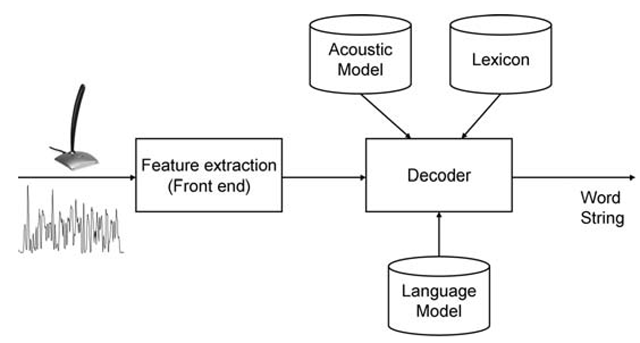
\includegraphics[scale=0.5]{tmp725d99_thumb}
%    \caption{Sphinx Architecture}
%    \label{fig:mesh1}
\end{figure}


\begin{figure}[h]
    \centering
    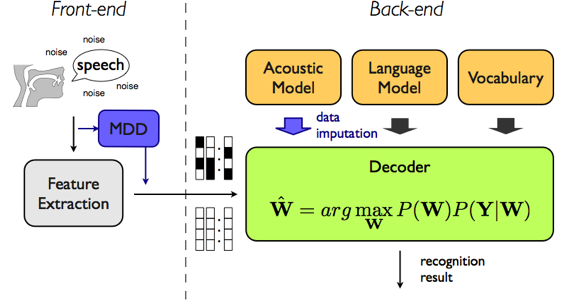
\includegraphics[scale=0.5]{mdt_recognizer}
    \caption{System Framework}
%    \label{fig:mesh1}
\end{figure}

%=====================================================================================================================================================
\chapter{EXPERIMENTAL RESULTS AND ANALYSIS}
\section{Platform}
\subsection{Operating System is Ubuntu 14.04}
Ubuntu is a Debian-based Linux operating system, with Unity as its default desktop environment. It is based on free software and named after the Southern African philosophy of ubuntu (literally, "human-ness"), which often is translated as "humanity towards others" or "the belief in a universal bond of sharing that connects all humanity".

Development of Ubuntu is led by UK-based Canonical Ltd. a company owned by South African entrepreneur Mark Shuttleworth. Canonical generates revenue through the sale of technical support and other services related to Ubuntu. The Ubuntu project is publicly committed to the principles of open-source software development; people are encouraged to use free software, study how it works, improve upon it, and distribute it [24].
\subsection{Bison}
Bison is a general-purpose parser generator that converts an annotated context-free grammar into a deterministic LR or generalized LR (GLR) parser employing LALR(1) parser tables. As an experimental feature, Bison can also generate IELR(1) or canonical LR(1) parser tables. Once you are proficient with Bison, you can use it to develop a wide range of language parsers, from those used in simple desk calculators to complex programming languages.

Bison is upward compatible with Yacc: all properly-written Yacc grammars ought to work with Bison with no change. Anyone familiar with Yacc should be able to use Bison with little trouble. You need to be fluent in C or C++ programming in order to use Bison. Java is also supported as an experimental feature [25].
\subsection{Swig}
To help build extension modules, SWIG is packaged with a library of support files that you can include in your own interfaces. These files often define new SWIG directives or provide utility functions that can be used to access parts of the standard C and C++ libraries. This chapter provides a reference to the current set of supported library files [26].
\subsection{Gstreamer} 
GStreamer is a pipeline-based multimedia framework written in the C programming language with the type system based on GObject.

GStreamer allows a programmer to create a variety of media-handling components, including simple audio playback, audio and video playback, recording, streaming and editing. The pipeline design serves as a base to create many types of multimedia applications such as video editors, streaming media broadcasters and media players.

It is designed to work on a variety of operating systems, e.g. Linux kernel-based operating systems, the BSDs, OpenSolaris, Android, OS X, iOS, Windows, OS/400.

GStreamer is free and open-source software subject to the terms of the GNU Lesser General Public License (LGPL) and is being hosted at freedesktop.org [27].
 	
GStreamer has been ported to a wide range of operating systems, processors and compilers. These include but are not limited to Linux on x86, PPC and ARM using GCC. Solaris on x86 and SPARC using both GCC and Forte, MacOSX, Microsoft Windows using MS Visual Developer, IBM OS/400 and Symbian OS.

GStreamer can bridge to other multimedia frameworks in order to reuse existing components (e.g. codecs) and use platform input/output mechanism [28].

\subsection{Gcc}
GCC was originally written as the compiler for the GNU operating system. The GNU system was developed to be 100 percent free software, free in the sense that it respects the user's freedom.

We strive to provide regular, high quality releases, which we want to work well on a variety of native and cross targets (including GNU/Linux), and encourage everyone to contribute changes or help testing GCC. Our sources are readily and freely available via SVN and weekly snapshots [27].

\subsection{Automake} 
Automake is a tool for automatically generating Makefile.in files compliant with the GNU Coding Standards. Automake requires the use of Autoconf [31]. The Automake manual can be read on-line or downloaded in PDF format; also, more formats are offered for download or on-line reading. If you have installed Automake on your system, you may also find more information about it by looking at your local documentation; for example you might use info automake at the shell prompt [27]. 
 
\subsection{Autoconf}
Autoconf is an extensible package of M4 macros that produce shell scripts to automatically configure software source code packages. These scripts can adapt the packages to many kinds of UNIX-like systems without manual user intervention. Autoconf creates a configuration script for a package from a template file that lists the operating system features that the package can use, in the form of M4 macro calls [28].

\subsection{Libtool}
 GNU libtool is a generic library support script. Libtool hides the complexity of using shared libraries behind a consistent, portable interface.

To use libtool, add the new generic library building commands to your Makefile, Makefile.in, or Makefile.am [28].




\section{Speech Recognition Engine}
\subsection{Library}
\subsubsection{Sphinxbase}
This package contains the basic libraries shared by the CMU Sphinx
trainer and all the Sphinx decoders (Sphinx-II, Sphinx-III, and
PocketSphinx), as well as some common utilities for manipulating
acoustic feature and audio files.

Sphinxbase uses the standard unix autogen system, and there's a script
included, 'build for iphone.sh' that will setup configure to create
binaries that are XCode friendly.

 ./autogen.sh

\subsubsection{Python-dev}
Header files, a static library and development tools for building
 Python modules, extending the Python interpreter or embedding Python
 in applications [20].

\subsection{Decoder}
\subsubsection{PocketSphinx}
 PocketSphinx is CMU’s fastest speech recognition system. It’s a library written in pure C which is optimal for development of your C applications as well as for development of language bindings. At real time speed it’s the most accurate engine, and therefore it is a good choice for live applications.

It's good for desktop applications, command and control and dictation where fast response and low resource consumption are the goals.

Also it includes support for embedded devices with fixed-point ariphmetics and is successfully used on IPhone, Nokia devices and on Windows Mobile. You can find further documentation about PocketSphinx in the release documentation, or at the online  documentation [29]. 

\subsubsection{Sphinx-4}
Sphinx-4 is a state-of-the-art speech recognition system written entirely in the Java™ programming language. It's best for implementation of complex server or cloud-based system with deep interaction with NLP modules, web services and cloud computing [29].

\subsection{Trainer}
\subsubsection{SphinxTrain}
 New openfst-based G2P trainer and decoder, supported by Sphinx4 too. It includes Parallel feature extraction.  Package can be installed now just like any application. Single 'sphinxtrain' command to access all training process. Increased reuse of sphinxbase functions [30].

\subsection{Experimental Setup}

\begin{enumerate}
  \item Installation of OS(operating system) i.e Ubuntu
  \item Install Bison 
  \item Install Swig
  \item Install Python-dev
  \item Install Automake 
  \item Install Autoconf
  \item Install Libtool
  \item Download Sphinxbase-5prealpha and compile it and then install from the source
  \item Download PocketSphinx-5prealpha and compile it and then install from the source
  \item Install Gstreamer  
  \item Download SphinxTrain-5prealpha and compile it and then install from the source	
\end{enumerate}

\section{Dictation System Setup}
Dictation system setup includes the making of Acoustic model and Language model for the Punjabi language. Also the use of CMULTK and testing on the PocketSphinx decoder.

\subsection{Testing the Decoder}
Before proceeding further it is important to check the existing decoder for the existing language model, so i test it with the exixting English model.
So i used Ubuntu terminal for this purpose.\\ 

\begin{figure}[h]
    \centering
    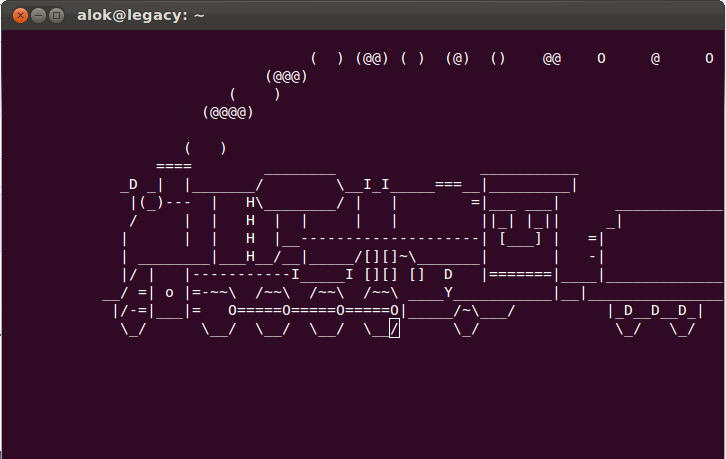
\includegraphics[scale=0.55]{networknuts-linux-fun}
    \caption{Ubuntu Terminal}
%    \label{fig:mesh1}
\end{figure}

The sphinxbase will be installed in /usr/local/ folder by default. Not every system loads libraries from this folder automatically. To load them you need to configure the path to look for shared libaries. It can be done either in the file /etc/ld.so.conf or with exporting environment variables:
\\
\textit{export LD\_LIBRARY\_PATH=/usr/local/lib} \\
\textit{export PKG\_CONFIG\_PATH=/usr/local/lib/pkgconfig}


To test installation, run 'pocketsphinx\_continuous -inmic yes' and check that it recognizes words you are saying to the microphone. 

\begin{figure}[h]
    \centering
    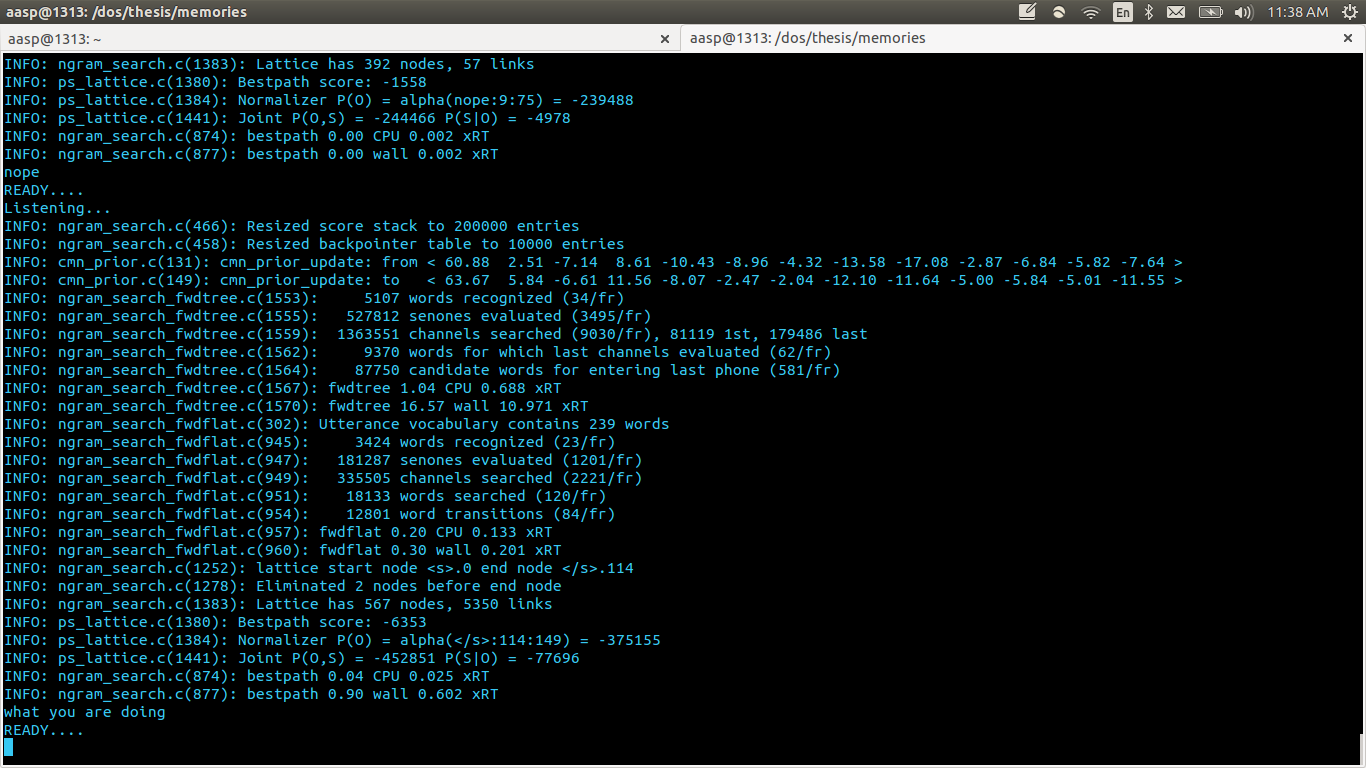
\includegraphics[scale=0.3]{Screenshot1}
    \caption{PocketSphinx Test}
%    \label{fig:mesh1}
\end{figure}

\subsection{Building Language Model}


There are two types of models that describe language - grammars and statistical language models. Grammars describe very simple types of languages for command and control, and they are usually written by hand or generated automatically with scripting code. Grammars usually do not have probabilities for word sequences, but some elements might be weighed. Grammars could be created with JSGF format and usually have extension like .gram or .jsgf.\\\\
Statistical language models describe more complex language. They contain probabilities of the words and word combinations. There are many ways to build the statistical language models. When your data set is large, there is sense to use CMU language modeling toolkit. When a model is small, you can use an online quick web service. When you need specific options or you just want to use your favorite toolkit which builds ARPA models, you can use it.
\\\\
Language model can be stored and loaded in two different format - text ARPA format and binary DMP format. ARPA format takes more space but it is possible to edit it. ARPA files have .lm extension. DMP format takes significantly less space and faster to load. DMP files have .lm.dmp extension. It is also possible to convert between formats.

\subsubsection{Text Preparation}
First of all you need to cleanup text. Expand abbreviations, convert numbers to words, clean non-word items. Language modeling for Mandarin is largely the same as in English, with one addditional consideration, which is that the input text must be word segmented. A segmentation tool and associated word list is provided to accomplish this. 
\subsubsection{ARPA Model Training}
The process for creating a language model is as follows:
\begin{enumerate}
  \item  Prepare a reference text that will be used to generate the language model. The language model toolkit expects its input to be in the form of normalized text files, with utterances delimited by <s> and </s> tags. A number of input filters are available for specific corpora such as Switchboard, ISL and NIST meetings, and HUB5 transcripts. The result should be the set of sentences that are bounded by the start and end sentence markers: <s> and </s>. Here's an example: 

\begin{figure}[h]
    \centering
    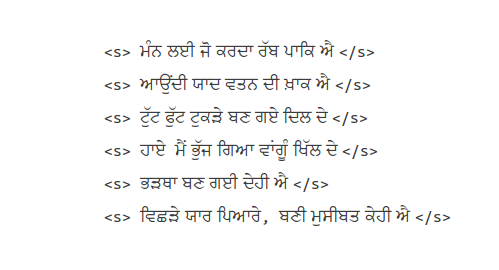
\includegraphics[scale=1.0]{Screenshot2}
    \caption{Text Prepration}
%    \label{fig:mesh1}
\end{figure}

More data will generate better language models. 

  \item  Generate the vocabulary file. This is a list of all the words in the file:

	\textit{text2wfreq < weather.txt | wfreq2vocab > weather.tmp.vocab} 
  \item Edit the vocabulary file to remove words (numbers, misspellings, names).
  \item Remove sentences from your input transcript that contain words that are not in your vocabulary file.
  \item Generate the arpa format language model with the commands:

	 \textit{text2idngram -vocab weather.vocab -idngram weather.idngram < weather.closed.txt \\
	 idngram2lm -vocab\_type 0 -idngram weather.idngram -vocab \ \\
     	 weather.vocab -arpa weather.lm}
  \item Generate the CMU binary form (DMP) 

	\textit{sphinx\_lm\_convert -i weather.lm -o weather.lm.DMP}
\end{enumerate}

\subsubsection{Using Language Model with PocketSphinx}

\textit{pocketsphinx\_continuous} can be run from the command-line to recognize speech. Assuming it is installed under \textit{/usr/local}, and your language model and dictionary are called \textit{.dic} and \textit{.lm} and placed in the current folder, try running the following command: 

\textit{pocketsphinx\_continuous -inmic yes -lm weather.lm -dict weather.dic}


\subsection{Training Acoustic Model For Sphinx}
CMUSphinx project comes with several high-quality acoustic models. Before starting with training we need to prepared the language model and  need to train the model and have resources to do that.

\subsubsection{Resources}
\begin{itemize}
 \item[$\bullet$] 1 hour of recording for command and control for single speaker
 \item[$\bullet$] 5 hour of recordings of 200 speakers for command and control for many speakers
 \item[$\bullet$] 10 hours of recordings for single speaker dictation
 \item[$\bullet$] 50 hours of recordings of 200 speakers for many speakers dictation
 \item[$\bullet$] Knowledge on phonetic structure of the language
 \item[$\bullet$] Time to train the model and optimize parameters (1 month)
\end{itemize}

\subsubsection{Data Preparation}

The trainer learns the parameters of the models of the sound units using a set of sample speech signals. This is called a training database. A choice of already trained databases will also be provided.\\\\
The database contains information required to extract statistics from the speech in form of the acoustic model.\\\\
The trainer needs to be told which sound units want it to learn the parameters of, and at least the sequence in which they occur in every speech signal in training database. This information is provided to the trainer through a file called the transcript file, in which the sequence of words and non-speech sounds are written exactly as they occurred in a speech signal, followed by a tag which can be used to associate this sequence with the corresponding speech signal.\\\\
The trainer then looks into a dictionary which maps every word to a sequence of sound units, to derive the sequence of sound units associated with each signal.\\\\
Thus, in addition to the speech signals, also be given a set of transcripts for the database (in a single file) and two dictionaries, one in which legitimate words in the language are mapped sequences of sound units (or sub-word units), and another in which non-speech sounds are mapped to corresponding non-speech or speech-like sound units. We will refer to the former as the language dictionary and the latter as the filler dictionary.\\\\
After training, it's mandatory to run the decoder to check training results. The Decoder takes a model, tests part of the database and reference transcriptions and estimates the quality (WER) of the model. During the testing stage we use the language model with the description of the order of words in the language.\\\\
First of all, design a database for training or download an existing one. For example, you can purchase a database from LDC. You'll have to convert it to a proper format. 

\textbf{The file structure for the database is:} 

\begin{description}
 \item[$\bigtriangledown$] etc
	\begin{description}
		\item[$\bullet$] some\_db.dic - \textit{Phonetic dictionary}
		\item[$\bullet$] some\_db.phone - \textit{Phoneset file}
		\item[$\bullet$] some\_db.lm.DMP - \textit{Language model}
		\item[$\bullet$] some\_db.filler - \textit{List of fillers}
		\item[$\bullet$] some\_db\_train.fileids - \textit{List of files for training}
		\item[$\bullet$] some\_db\_train.transcription - \textit{Transcription for training}
		\item[$\bullet$] some\_db\_test.fileids - \textit{List of files for testing}
		\item[$\bullet$] some\_db\_test.transcription - \textit{Transcription for testing}
		\item[$\bullet$] some\_
		\item[$\bullet$] some\_
	\end{description}
 \item[$\bigtriangledown$] wav
	\begin{description}
		\item[$\bigtriangledown$] speaker\_1
			\begin{description}
				\item[$\bullet$] file\_1.wav - \textit{Recording of speech utterance}
			\end{description}
		\item[$\bigtriangledown$] speaker\_2
			\begin{description}
				\item[$\bullet$]file\_2.wav
			\end{description}
	\end{description}	
\end{description}



\textit{Fileids (some\_db\_train.fileids and some\_db\_test.fileids)} file is a text file listing the names of the recordings (utterance ids) one by line.
\\\\
\textit{Transcription file (your\_db\_train.transcription and your\_db\_test.transcription)} is a text file listing the transcription for each audio file. t's important that each line starts with <s> and ends with </s> followed by id in parentheses. Also note that parenthesis contains only the file, without speaker\_n directory. It's critical to have exact match between fileids file and the transcription file. The number of lines in both should be identical. Last part of the file id (speaker1/file\_1) and the utterance id file\_1 must be the same on each line.\\\\
Speech recordings (wav files) Recording files must be in MS WAV format with specific sample rate - 16 kHz, 16 bit, mono for desktop application, 8kHz, 16bit, mono for telephone applications. Double-check that, wrong audio file format is the most common source of training issues. Audio files shouldn't be very long and shouldn't be very short. Optimal length is not less than 5 seconds and not more than 30 seconds. Amount of silence in the beginning of the utterance and in the end of the utterance should not exceed 0.2 second. \\\\
\textit{Phoneset file (your\_db.phone)} should have one phone per line. The number of phones should match the phones used in the dictionary plus the special SIL phone for silence.\\\\
\textit{Language model file (your\_db.lm.DMP)} should be in ARPA format or in DMP format. 
\textit{Filler dictionary (your\_db.filler)} contains filler phones (not-covered by language model non-linguistic sounds like breath, hmm or laugh).\\\\
\subsubsection{Setting up the training scripts}
To start the training change to the database folder and run the following commands:\\\\
\textit{sphinxtrain -t <model\_name> setup}\\\\

This will copy all the required configuration files into etc subfolder of your database folder and prepare database for training, the structure after setup will be: 
\begin{itemize}
  \item[$\bullet$] etc
  \item[$\bullet$] wav
\end{itemize}

After training other data folders will be created, the database should look like this: 

\begin{itemize}
	
  \item[$\triangleright$] etc
  \item[$\triangleright$] feat 
  \item[$\triangleright$] logdir
  \item[$\triangleright$]model\_parameters
  \item[$\triangleright$]model\_architecture
  \item[$\triangleright$]result
  \item[$\triangleright$]wav
%  \item[$\triangleright$]
%  \item[$\triangleright$]
\end{itemize}


\subsubsection{Setup the Format of Database Audio}
After setup, we need to edit the configuration files in etc folder, there are many variables but to get started we need to change only a few. First of all find the file \textit{etc/sphinx\_train.cfg}\\
\textit{
\$CFG\_WAVFILES\_DIR = "\$CFG\_BASE\_DIR/wav";\\
\$CFG\_WAVFILE\_EXTENSION = 'sph';\\
\$CFG\_WAVFILE\_TYPE = 'nist';  one of nist, mswav, raw
}

\subsubsection{Configure Path to Files}
 See the following lines in your etc/sphinx\_train.cfg file:\\
\textit{ 
\$CFG\_DICTIONARY     = "\$CFG\_LIST\_DIR/\$CFG\_DB\_NAME.dic";\\
\$CFG\_RAWPHONEFILE   = "\$CFG\_LIST\_DIR/\$CFG\_DB\_NAME.phone";\\
\$CFG\_FILLERDICT     = "\$CFG\_LIST\_DIR/\$CFG\_DB\_NAME.filler";\\
\$CFG\_LISTOFFILES    = "\$CFG\_LIST\_DIR/\${CFG\_DB\_NAME}\_train.fileids";\\
\$CFG\_TRANSCRIPTFILE = "\$CFG\_LIST\_DIR/\${CFG\_DB\_NAME}\_train.transcription"
}

\subsubsection{Configure Model Type and Model Parameters}
\textit{
\$CFG\_HMM\_TYPE = '.cont.'; \# Sphinx4, Pocketsphinx\\
\#\$CFG\_HMM\_TYPE  = '.semi.'; \# PocketSphinx only\\
\#\$CFG\_HMM\_TYPE  = '.ptm.'; \# Sphinx4, Pocketsphinx, faster model\\
}


If you are training continuous models for large vocabulary and have more than 100 hours of data, put 32 here. It can be any degree of 2: 4, 8, 16, 32, 64. 
\textit{\$CFG\_FINAL\_NUM\_DENSITIES = 8;}\\

This value is the number of senones to train in a model. The more senones model has, the more precisely it discriminates the sounds. But on the other hand if you have too many senones, model will not be generic enough to recognize unseen speech. That means that the WER will be higher on unseen data. That's why it is important to not overtrain the models. In case there are too many unseen senones, the warnings will be generated in the norm log on stage 50 below: 
\textit{
ERROR: "gauden.c", line 1700: Variance (mgau= 948, feat= 0, density=3, \\
component=38) is less then 0. Most probably the number of senones is too\\
high for such a small training database. Use smaller \$CFG\_N\_TIED\_STATES.}

\begin{table}
\centering
\caption{Continuous Model Senones and Density}
\begin{tabular}
{ |p{2cm}||p{2cm}|p{2cm}|p{2cm}|p{3cm}|  }
 \hline

 \multicolumn{5}{|c|}{Number of Senones and Number of Densities} \\
 \hline
 Vocabulary  &  Hours in db  & Senones &  Densities & Example \\
 \hline
 20 &	5    &	200  &	8  &	Tidigits Digits Recognition\\
\hline
100 &	20   &	2000 &	8  &	RM1 Command and Control\\
\hline
5000 &	30   &	4000 &	16 &	WSJ1 5k Small Dictation\\
\hline
20000 &	80   &	4000 &	32 &	WSJ1 20k Big Dictation\\
\hline
60000 &	200  &	6000 &	16 &	HUB4 Broadcast News\\
\hline
60000 &	2000 &	12000 &	64 &	Fisher Rich Telephone Transcription\\

 \hline

\end{tabular}
\end{table}


It might seem that diversity could improve the model but it's not the case. Diverse speech requires some artificial speech prompts and that decrease the naturalness of the speech. Artificial models don't help in real life decoding. In order to build a best database you need to try to reproduce real environment as much as possible. It's even better to collect more speech to try to optimize the database size.

It's important to remember, that optimal numbers depends on your database. To train model properly, you need to experiment with different values and try to select the ones which give best WER for a development set. You can experiment with number of senones, number of gaussian mixtures at least. Sometimes it's also worth to experiment with phoneset or number of estimation iterations. 

\subsubsection{Configure Sound Feature Parameters}
The default for sound files used in Sphinx is a rate of 16 thousand samples per second (16KHz). If this is the case, the etc/feat.params file will be automatically generated with the recommended values. \\
\textit{
\# Feature extraction parameters
\$CFG\_WAVFILE\_SRATE = 16000.0;\\
\$CFG\_NUM\_FILT = 31; \# For wideband speech it's 40, for telephone 8khz reasonable value is 31\\
\$CFG\_LO\_FILT = 200; \# For telephone 8kHz speech value is 200\\
\$CFG\_HI\_FILT = 3500; \# For telephone 8kHz speech value is 3500\\
}

\subsubsection{Configure Parallel Jobs to Speedup Training}
If you are on multicore machine or in PBS cluster you can run training in parallel, the following options should do the trick: \\
\textit{
\# Queue::POSIX for multiple CPUs on a local machine
\# Queue::PBS to use a PBS/TORQUE queue
\$CFG\_QUEUE\_TYPE = "Queue";
}

\subsubsection{Configure Decoding Parameters}
Open \textit{etc/sphinx\_train.cfg}, make sure the following is properly configured:\\
\textit{
\$DEC\_CFG\_DICTIONARY     = "\$DEC\_CFG\_BASE\_DIR/etc/\$DEC\_CFG\_DB\_NAME.dic";
}\\
\textit{\$DEC\_CFG\_FILLERDICT     = "\$DEC\_CFG\_BASE\_DIR/etc/\$DEC\_CFG\_DB\_NAME.filler";}
\textit{\$DEC\_CFG\_LISTOFFILES    = "\$DEC\_CFG\_BASE\_DIR/etc/\${DEC\_CFG\_DB\_NAME}\_test.fileids";}
\textit{\$DEC\_CFG\_TRANSCRIPTFILE = "\$DEC\_CFG\_BASE\_DIR/etc/\\ \${DEC\_CFG\_DB\_NAME}\_test.transcription";}\\
\textit{\$DEC\_CFG\_RESULT\_DIR     = "\$DEC\_CFG\_BASE\_DIR/result";}\\
\# These variables, used by the decoder, have to be user defined, and\\
\# may affect the decoder output\\
\textit{\$DEC\_CFG\_LANGUAGEMODEL\_DIR = "\$DEC\_CFG\_BASE\_DIR/etc";}\\
\textit{\$DEC\_CFG\_LANGUAGEMODEL  = "\$DEC\_CFG\_LANGUAGEMODEL\_DIR\\/model\_name.lm.DMP";}

\subsubsection{Training}
 First of all, go to the database directory: 
\textit{cd some\_dir}

To train, just run the following commands: 

\textit{sphinxtrain run}

and it will go through all the required stages. It will take a few minutes to train. On large databases, training could take a month.
During the stages, the most important stage is the first one which checks that everything is configured correctly and your input data is consistent. Do not ignore the errors reported on the first 00.verify\_all step.

 The typical output during decoding will look like: 

\begin{figure}[h]
    \centering
    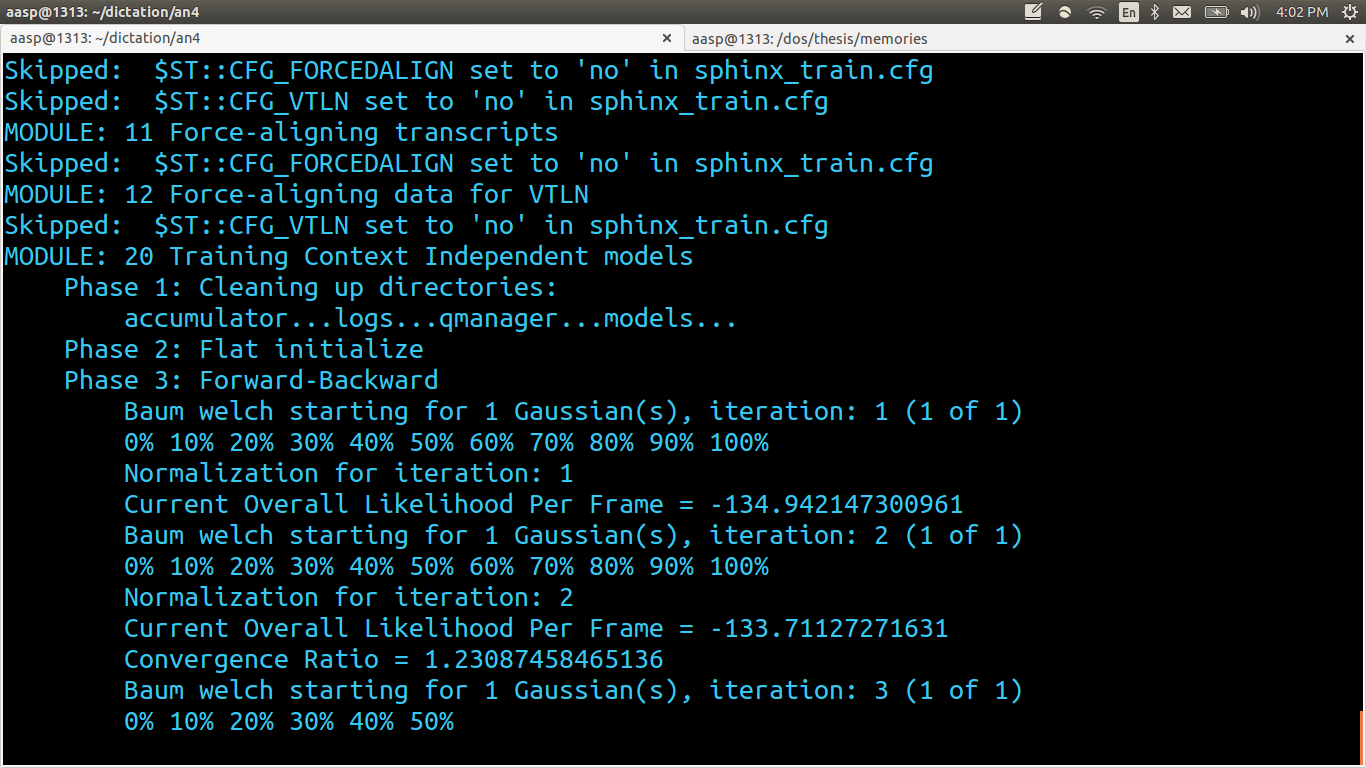
\includegraphics[scale=0.3]{Screenshot3}
    \caption{Training Model}
%    \label{fig:mesh1}
\end{figure}

\subsubsection{Training Internals}
This section describes what happens during the training. In the scripts directory (./scripts\_pl), there are several directories numbered sequentially from 00 through 99. Each directory either has a directory named slave*.pl or it has a single file with extension .pl. The script sequentially goes through the directories and executes either the the slave*.pl or the single .pl file, as below. \\
\textit{
perl scripts\_pl/000.comp\_feat/slave\_feat.pl\\
perl scripts\_pl/00.verify/verify\_all.pl\\
perl scripts\_pl/10.vector\_quantize/slave.VQ.pl\\
perl scripts\_pl/20.ci\_hmm/slave\_convg.pl\\
perl scripts\_pl/30.cd\_hmm\_untied/slave\_convg.pl\\
perl scripts\_pl/40.buildtrees/slave.treebuilder.pl\\
perl scripts\_pl/45.prunetree/slave-state-tying.pl\\
perl scripts\_pl/50.cd\_hmm\_tied/slave\_convg.pl\\
perl scripts\_pl/90.deleted\_interpolation/deleted\_interpolation.pl\\
}


 Scripts launch jobs on your machine, and the jobs will take a few minutes each to run through.

Before you run any script, note the directory contents of your current directory. After you run each slave*.pl note the contents again. Several new directories will have been created. These directories contain files which are being generated in the course of your training. At this point you need not know about the contents of these directories, though some of the directory names may be self explanatory and you may explore them if you are curious.

One of the files that appears in your current directory is an .html file, named model.html, depending on which database you are using. This file will contain a status report of jobs already executed. Verify that the job you launched completed successfully. Only then launch the next slave*.pl in the specified sequence. Repeat this process until you have run the slave*.pl in all directories.

Note that in the process of going through the scripts in 00* through 90*, you will have generated several sets of acoustic models, each of which could be used for recognition. Notice also that some of the steps are required only for the creation of semi-continuous models. If you execute these steps while creating continuous models, the scripts will benignly do nothing. 

 On the stage 000.comp\_feat the feature feles are extracted. The system does not directly work with acoustic signals. The signals are first transformed into a sequence of feature vectors, which are used in place of the actual acoustic signals.

This script slave\_feat.pl will compute, for each training utterance, a sequence of 13-dimensional vectors (feature vectors) consisting of the Mel-frequency cepstral coefficients (MFCCs). Note that the list of wave files contains a list with the full paths to the audio files. Since the data are all located in the same directory as you are working, the paths are relative, not absolute. You may have to change this, as well as the model\_test.fileids file, if the location of data is different. The MFCCs will be placed automatically in a directory called 'feat'. Note that the type of features vectors you compute from the speech signals for training and recognition, outside of this tutorial, is not restricted to MFCCs. You could use any reasonable parameterization technique instead, and compute features other than MFCCs. CMUSphinx can use features of any type or dimensionality. The format of the features is described on the page MFC Format . 

\subsubsection{Testing}
 It's critical to test the quality of the trained database in order to select best parameters, understand how application performs and optimize performance. To do that, a test decoding step is needed. The decoding is now a last stage of the training process.

You can restart decoding with the following command: 
\textit{sphinxtrain -s decode run}
 This command will start a decoding process using the acoustic model you trained and the language model you configured in the \textit{etc/sphinx\_train.cfg} file.

\begin{figure}[h]
    \centering
    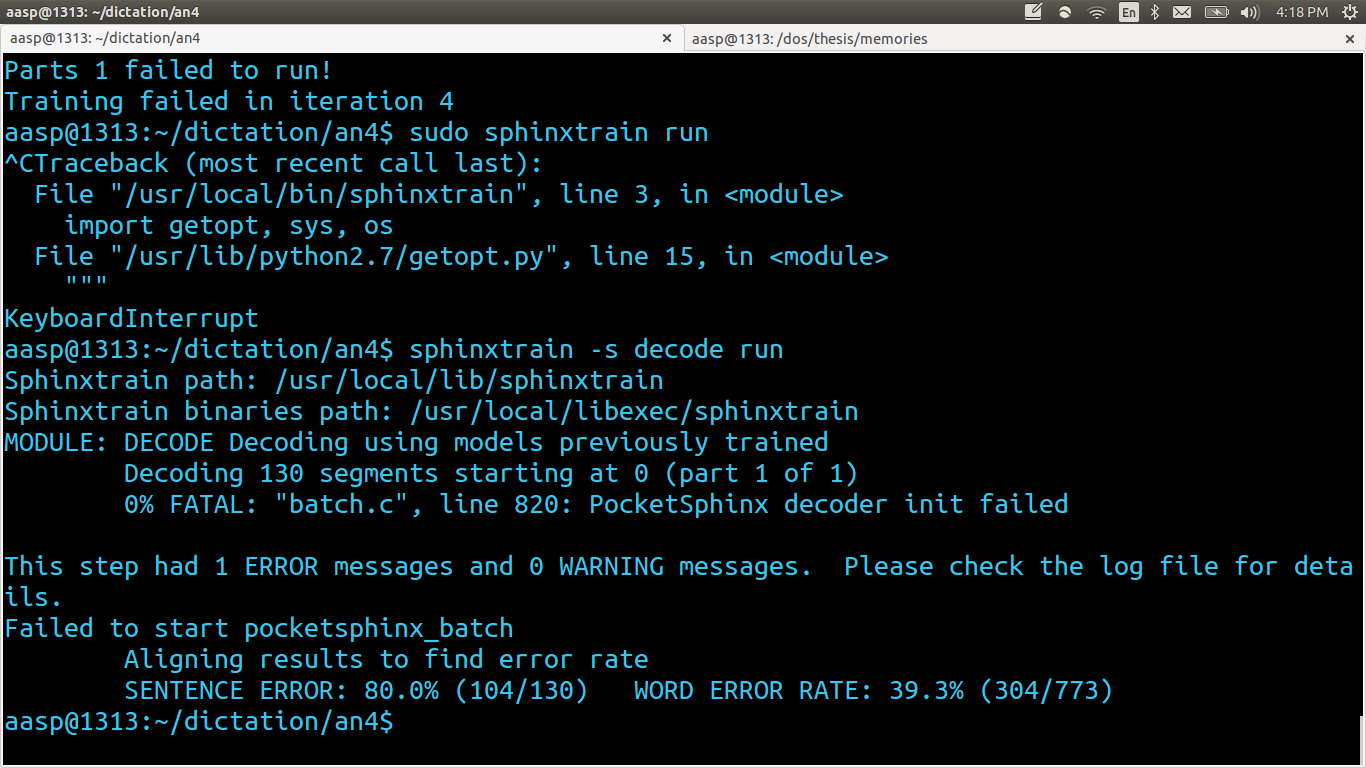
\includegraphics[scale=0.3]{Screenshot4}
    \caption{Testing Model}
%    \label{fig:mesh1}
\end{figure}

\subsubsection{Using the Model}
After training, the acoustic model is located in \\

\textit{model\_parameters/<your\_db\_name>.cd\_cont\_<number\_of senones>}

or in 

\textit{model\_parameters/<your\_db\_name>.cd\_semi\_<number\_of senones>}

The model should have the following files:
\begin{itemize}
	\item[$\bullet$] mdef
	\item[$\bullet$] feat.params
	\item[$\bullet$]mixture\_weights
	\item[$\bullet$]means
	\item[$\bullet$]noisedict
	\item[$\bullet$]transition\_matrices
	\item[$\bullet$]variances
\end{itemize}

Depending on the type of the model you trained. To use the model in pocketsphinx, simply point to it with the -hmm option: \\\\

\textit{pocketsphinx\_continuous -hmm <model\_folder> -lm <some\_lm> -dict <some\_dict>.}

\subsubsection{Output}

The output the model trained for Punjabi language is given in the figure below:



\begin{figure}[h]
    \centering
    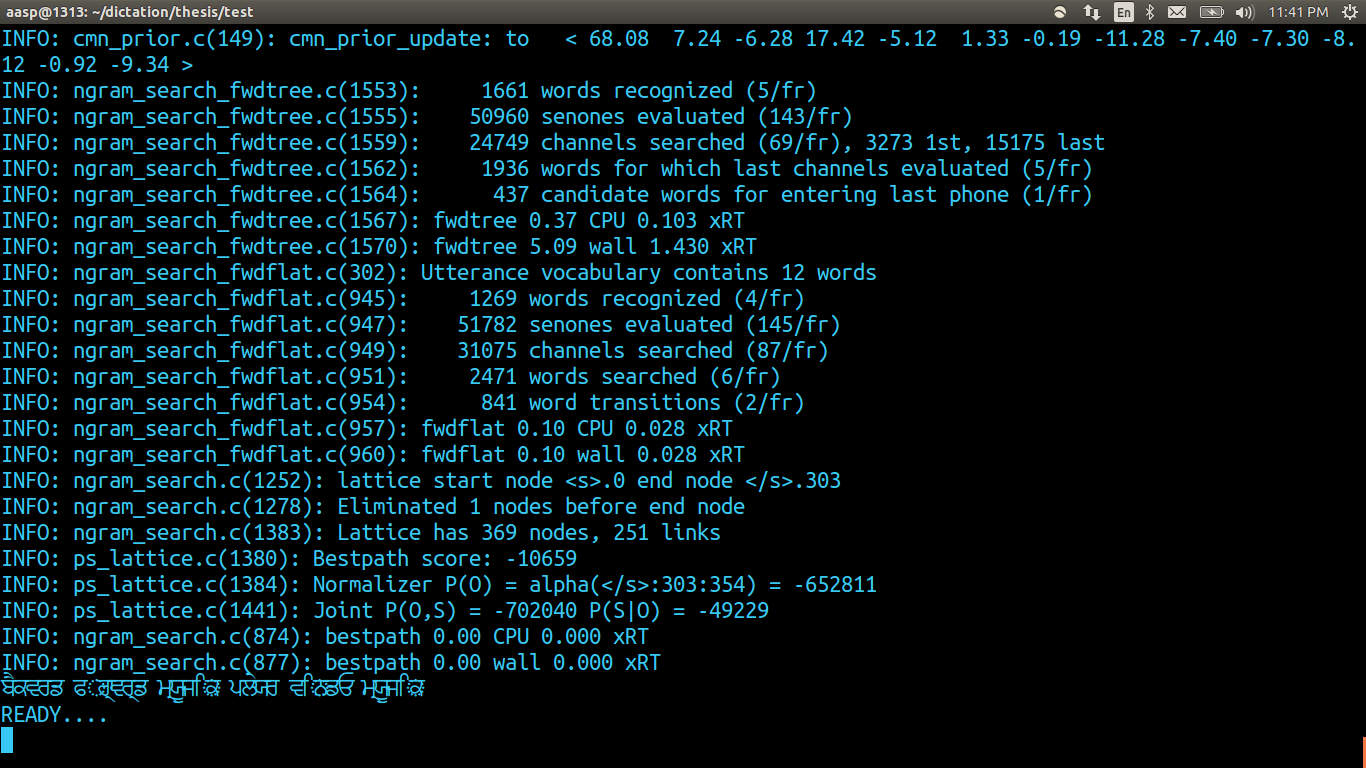
\includegraphics[scale=0.3]{Screenshot5}
    \caption{Punjabi Dictation}
%    \label{fig:mesh1}
\end{figure}

\begin{figure}[h]
    \centering
    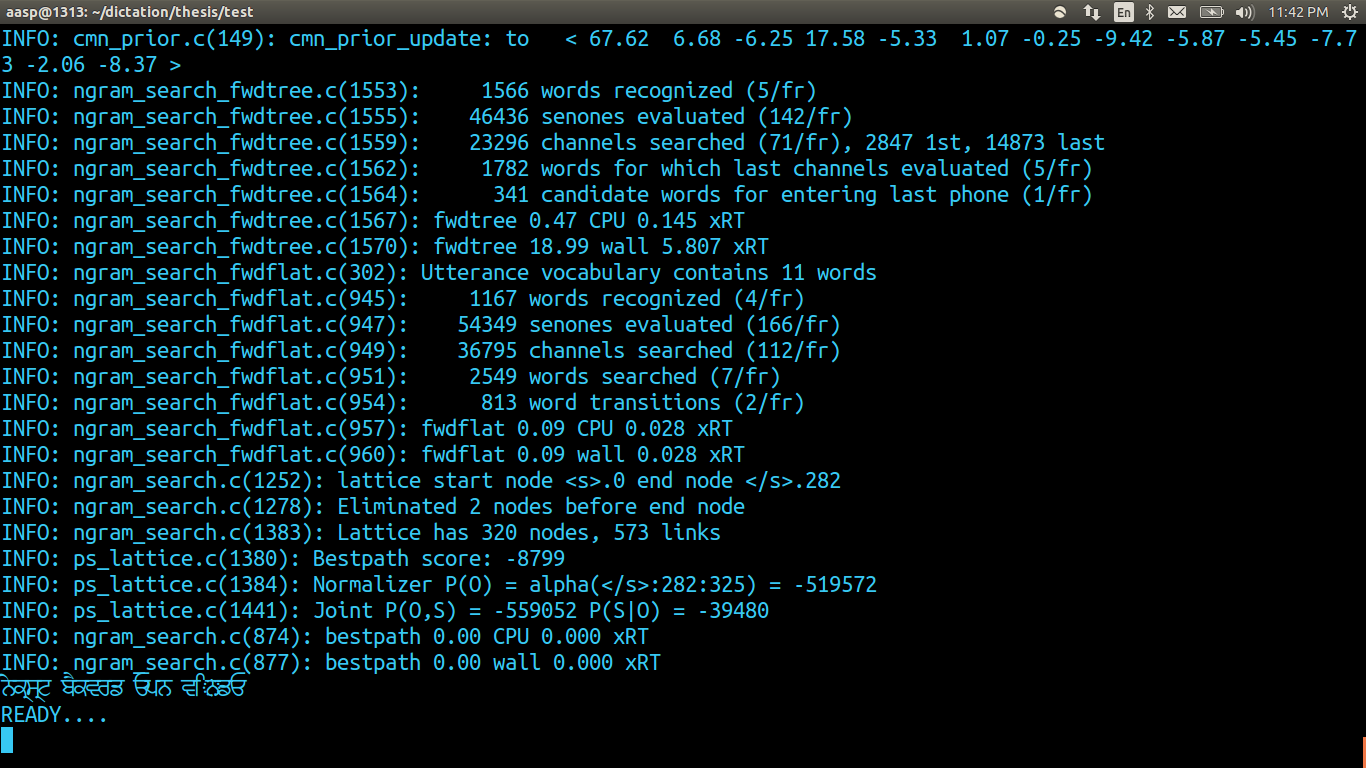
\includegraphics[scale=0.3]{Screenshot6}
    \caption{punjabi Dictation}
%    \label{fig:mesh1}
\end{figure}


%=====================================================================================================================================================
\chapter{CONCLUSION}

\section{Conclusion}
For the past many years, several mechanisms for the communication among human-
machine have been explored. There is much evidence that human speech dictation in
machine involves the integration of a great variety of knowledge sources, including
knowledge of the world or context, knowledge of the speaker and/or topic and many
more. Although there have been significant recent gains in speech dictation, current
technology is far from human-like: only systems in limited domains can be envisioned
in the near term, and the portability of existing techniques is still rather limited.
Application areas that appear to be a good match to technology on the near horizon
include those that are naturally limited.

The objective of the thesis was “speech pattern recognition for speech to text
conversion”. The researcher desire was to pronounced the Punjabi character from any
user, identify it and print it in the text editor. In other word, the recognition of the
Punjabi character or one can say the dictation of the Punjabi character.

\section{Future Work}

The speech dictation is a very huge research work area and required a team of skilled
researcher. Although, the researcher has tried his level best to detect the Punjabi
character. When the idea of the speech dictation was born in the mind of the
researcher, his dream was to dictate the Punjabi continuous speech. The work is of
considerable domain and hence the beginning to end of the work has made with the
detection of Punjabi characters and with its total analysis. So the present study has scope for the
continuation of research for all the remaining Punjabi characters, which further can
be extended in the Punjabi word dictation and ultimately the dictation of words can
again be extended for the continuous speech dictation in Punjabi language.

Although many recent advances and successes in speaker recognition have been
achieved, there are still many possible enhancement for which good solutions are to
be found. Most of these problems arise from variability, including speaker-generated
variability and variability in channel and recording conditions. It is very important to
investigate feature parameters that are stable over time, insensitive to the variation of
speaking manner, including the speaking rate and level, and robust against variations
in voice quality due to causes such as voice disguise or colds and many more ...









%%%%%%%%%%%%%%%%%%%%%%%%%%%%%%%%%%%%%%%%%%%%%%%%%%%%%%%%%%%%%%%%%%%%%%%%%%%%%%%%%%%%%%%%%%%%%%%%%%%%%%%%%%%%%%%%%%%%%%%%%%%%%%%%%%%%%%%%%%%%%%%%%%


%\appendix

%\chapter{Additional}
%Lorem ipsum dolor sit amet, consectetur adipiscing elit, sed do eiusmod tempor incididunt ut labore et dolore magna aliqua. Ut enim ad minim veniam, quis nostrud exercitation ullamco laboris nisi ut aliquip ex ea commodo consequat. Duis aute irure dolor in reprehenderit in voluptate velit esse cillum dolore eu fugiat nulla pariatur. Excepteur sint occaecat cupidatat non proident, sunt in culpa qui officia deserunt mollit anim id est laborum.
%%%%%%%%%%%%%%%%%%%%%%%%%%%%%%%%%%%%%%%%%%%%%%%%%%%%%%%%%%%%%%%%%%%%%%%%%%%%%%%%%%%%%%%%%%%%%%%%%%%%%%%%%%%%%%%%%%%%%%%%%%%%%%%%%%%%%%%%%%%%%%%%%%


%=====================================================================================================================================================


%\bibliographystyle{unsrt}
%\bibliography{sample}

%\printbibliography[title=References]


\begin{thebibliography}{9}

\bibitem{1}
Chowdhury, Gobinda G. 
"Natural language processing."
%Annual review of information science and technology 37.1 (2003): 51­89.
\textit{Annual review of information science and technology 37.1,} 2003: 5189.

\bibitem{2}
Kaur, Navdeep,Vandana Pushe, and Rupinderdeep Kaur.
Natural Language Processing Interface for Synonym."
\textit{from outside the contents of the document,} 2014.

\bibitem{3}
Kaur, Kamaldeep, and Vishal Gupta.
"Name and Entity Recognition for Punjabi Language."
\textit{Machine translation 2.3,} 2012.

\bibitem{4}Necula, George C."Translation validation for an optimizing compiler."
\textit{ACM sigplan notices. Vol. 35. No. 5. ACM,} 2000.


\bibitem{5}Mac, David, Tom, and Alexendre. "GNU Automake."
\textit{User Manual, for Automake version 1,} 1995.

\bibitem{6} Calcote, John. "Autotools: A Practitioner's"
\textit{Guide to GNU Autoconf, Automake, and Libtool. No Starch Press,} 2010.

\bibitem{7}Byrne, William, et al. "Towards language independent acoustic modeling."
\textit{Acoustics, Speech, and Signal Processing,} 2000. ICASSP'00. Proceedings. 2000 IEEE International Conference on. Vol. 2. IEEE, 2000.

\bibitem{8}Lippmann, Richard P. "Speech recognition by machines and humans."
\textit{Speech communication 22.1,} 1997.

\bibitem{9} Schultz, TAnja, and Alex. "Language independent and languge adaptive acoustic model for speech recognition."
\textit{Speech Communication 35.1,} 2001.

\bibitem{10} Walker, Willie, et al. "Sphinx4: A flexible open source framework for speech recognition,", 2004.
\textit{}

\bibitem{11}Sankar, Fuliang Weng Andreas Stolcke Ananth. "Efficient Lattice Representation and Generation.", 2006.
\textit{}

\bibitem{12} Dua, Mohit, et al. "Punjabi automatic speech recognition using HTK."
\textit{IJCSI International Journal of Computer Science Issues 9.4,} 2012.


\bibitem{13} Ravinder, Kumar. "Comparison of hmm and dtw for isolated word recognition system of punjabi language."
\textit{Progress in Pattern Recognition, Image Analysis, Computer Vision, and Applications. Springer Brelin,} 2010.

\bibitem{14}Grasch, Peter, Alexander Felfernig, and Florian Reinfrank. "ReComment: Towards critiquing-
based recommendation with speech interaction."
\textit{Proceedings of the 7th ACM Conference on Recommender Systems. ACM,} 2013.

\bibitem{15}Ravinder, and Rajendra Kumar Sharma. "An efficient post processing algorithm for online handwriting Gurmukhi character recognition using set theory."
\textit{International Journal of Pattern Recognition and Artificial Intelligence 27.04,} 2013.

\bibitem{16}Bansal, Divya, Ankita Goel, and Khushneet Jindal. "Punjabi Speech Synthesis System Using Htk."
\textit{International Journal of Information 2.4,} 2012.

\bibitem{17}Dua, Mohit, et al. "Punjabi speech to text system for connected words.", 2012.
\textit{}

\bibitem{18}Ghai, Wiqas, and Navdeep Singh. "Continuous Speech Recognition for Punjabi."2013.
\textit{}

\bibitem{19}
http://www.programmershare.com/
%\textit{}

\bibitem{20}
http://cmusphinx.sourceforge.net/wiki/
%\textit{}

\bibitem{21}
[6]Kumbharana, Chandresh K."Speech Pattern Recognition for Speech to Text Conversion."
\textit{Diss. Saurashtra University,} 2007.

\bibitem{22} Electronics for U may 2000
%\textit{}

\bibitem{23}IBM, Developing voice applications.
%\textit{}

\bibitem{24} https://en.wikipedia.org/wiki/Ubuntu\_(28operating\_system)
\textit{}

\bibitem{25}http://www.gnu.org/software/bison/
\textit{}

\bibitem{26}http://www.swig.org/Doc1.3/Library.html
\textit{}

\bibitem{27}https://en.wikipedia.org/wiki/GStreamer
\textit{}

\bibitem{28}http://gstreamer.freedesktop.org/features/
\textit{}

\bibitem{29}https://launchpad.net/ubuntu/precise/+package/pythondev
\textit{}

\bibitem{30}http://sourceforge.net/projects/cmusphinx/files/sphinxtrain/5prealpha/
\textit{}

\bibitem{31}https://www.gnu.org/software/automake/
\textit{}



\end{thebibliography}




\end{document}

